%%%%%%%%%%%%% TO run it - create a new Project in Rstudio - from existing folder - specify this poster folder
%%%
%%%%%%%%%%%%%%%%%%%%%%%%%%%%%%%%%%%%%%%%%
% a0poster Landscape Poster
% LaTeX Template
% Version 1.0 (22/06/13)
%
% The a0poster class was created by:
% Gerlinde Kettl and Matthias Weiser (tex@kettl.de)
% 
% This template has been downloaded from:
% http://www.LaTeXTemplates.com
%
% License:
% CC BY-NC-SA 3.0 (http://creativecommons.org/licenses/by-nc-sa/3.0/)
%
%%%%%%%%%%%%%%%%%%%%%%%%%%%%%%%%%%%%%%%%%

%----------------------------------------------------------------------------------------
%	PACKAGES AND OTHER DOCUMENT CONFIGURATIONS
%----------------------------------------------------------------------------------------

\documentclass[a0,landscape]{a0poster}\usepackage[]{graphicx}\usepackage[]{color}
%% maxwidth is the original width if it is less than linewidth
%% otherwise use linewidth (to make sure the graphics do not exceed the margin)
\makeatletter
\def\maxwidth{ %
  \ifdim\Gin@nat@width>\linewidth
    \linewidth
  \else
    \Gin@nat@width
  \fi
}
\makeatother

\definecolor{fgcolor}{rgb}{0.345, 0.345, 0.345}
\newcommand{\hlnum}[1]{\textcolor[rgb]{0.686,0.059,0.569}{#1}}%
\newcommand{\hlstr}[1]{\textcolor[rgb]{0.192,0.494,0.8}{#1}}%
\newcommand{\hlcom}[1]{\textcolor[rgb]{0.678,0.584,0.686}{\textit{#1}}}%
\newcommand{\hlopt}[1]{\textcolor[rgb]{0,0,0}{#1}}%
\newcommand{\hlstd}[1]{\textcolor[rgb]{0.345,0.345,0.345}{#1}}%
\newcommand{\hlkwa}[1]{\textcolor[rgb]{0.161,0.373,0.58}{\textbf{#1}}}%
\newcommand{\hlkwb}[1]{\textcolor[rgb]{0.69,0.353,0.396}{#1}}%
\newcommand{\hlkwc}[1]{\textcolor[rgb]{0.333,0.667,0.333}{#1}}%
\newcommand{\hlkwd}[1]{\textcolor[rgb]{0.737,0.353,0.396}{\textbf{#1}}}%

\usepackage{framed}
\makeatletter
\newenvironment{kframe}{%
 \def\at@end@of@kframe{}%
 \ifinner\ifhmode%
  \def\at@end@of@kframe{\end{minipage}}%
  \begin{minipage}{\columnwidth}%
 \fi\fi%
 \def\FrameCommand##1{\hskip\@totalleftmargin \hskip-\fboxsep
 \colorbox{shadecolor}{##1}\hskip-\fboxsep
     % There is no \\@totalrightmargin, so:
     \hskip-\linewidth \hskip-\@totalleftmargin \hskip\columnwidth}%
 \MakeFramed {\advance\hsize-\width
   \@totalleftmargin\z@ \linewidth\hsize
   \@setminipage}}%
 {\par\unskip\endMakeFramed%
 \at@end@of@kframe}
\makeatother

\definecolor{shadecolor}{rgb}{.97, .97, .97}
\definecolor{messagecolor}{rgb}{0, 0, 0}
\definecolor{warningcolor}{rgb}{1, 0, 1}
\definecolor{errorcolor}{rgb}{1, 0, 0}
\newenvironment{knitrout}{}{} % an empty environment to be redefined in TeX

\usepackage{alltt}

\usepackage{multicol} % This is so we can have multiple columns of text side-by-side
\columnsep=100pt % This is the amount of white space between the columns in the poster
\columnseprule=3pt % This is the thickness of the black line between the columns in the poster

\usepackage[svgnames]{xcolor} % Specify colors by their 'svgnames', for a full list of all colors available see here: http://www.latextemplates.com/svgnames-colors

\usepackage{times} % Use the times font
%\usepackage{palatino} % Uncomment to use the Palatino font

\usepackage{graphicx} % Required for including images
\graphicspath{{figures/}} % Location of the graphics files
\usepackage{booktabs} % Top and bottom rules for table
\usepackage[font=small,labelfont=bf]{caption} % Required for specifying captions to tables and figures
\usepackage{amsfonts, amsmath, amsthm, amssymb} % For math fonts, symbols and environments
\usepackage{wrapfig} % Allows wrapping text around tables and figures
\usepackage{caption}
\usepackage{lipsum}
\IfFileExists{upquote.sty}{\usepackage{upquote}}{}
\begin{document}
%\SweaveOpts{concordance=TRUE}

%----------------------------------------------------------------------------------------
%	POSTER HEADER 
%----------------------------------------------------------------------------------------

% The header is divided into three boxes:
% The first is 55% wide and houses the title, subtitle, names and university/organization
% The second is 25% wide and houses contact information
% The third is 19% wide and houses a logo for your university/organization or a photo of you
% The widths of these boxes can be easily edited to accommodate your content as you see fit

\begin{minipage}[b]{0.65\linewidth}
\veryHuge \color{NavyBlue} \textbf{Correlations between emotional factors and the stock market} \color{Black}\\ \\% Title
\huge \textbf{Max Xiong}\\ % Author(s)
\huge Data Science Research Laboratory. Mentor: Dr. S. Samsonau\\ % Subtitle
\huge Princeton International School of Mathematics and Science\\ % University/organization
\end{minipage}
%
\begin{minipage}[b]{0.2\linewidth}
\color{DarkSlateGray}\Large \textbf{Address and Contact Information:}\\
19 Lambert Dr, Princeton NJ 08540\\ % Address
e-mail: \texttt{Max.Xiong@prismsus.org}\\ % Email address
\end{minipage}
%
\begin{minipage}[b]{0.14\linewidth}

\includegraphics[width=13cm]{PRISMS_Logo.jpg} % Logo or a photo of you, adjust its dimensions here
\end{minipage}

\vspace{1cm} % A bit of extra whitespace between the header and poster content

%----------------------------------------------------------------------------------------

\begin{multicols}{4} % This is how many columns your poster will be broken into, a poster with many figures may benefit from less columns whereas a text-heavy poster benefits from more

%----------------------------------------------------------------------------------------
%	ABSTRACT
%----------------------------------------------------------------------------------------

\color{Navy} % Navy color for the abstract

\begin{abstract}

When people talk about stock market, they most likely relate it to the pure number analysis such as operation profitability, debt equity ratio, dividends for investors, etc. Nowadays, computer algorithm controls more than fifty percent of the trading volume so humans seem less important in the process than they were in the past. However, the large amount of capital invested by normal investors are still considerable. In order to analyze what may possibly influence the decisions made by traditional investors, this research studies the emotion factors in investment, as information is the fundamental criteria for normal investors, by quantifying the emotional levels

\end{abstract}

%----------------------------------------------------------------------------------------
%	INTRODUCTION
%----------------------------------------------------------------------------------------

\color{SaddleBrown} % SaddleBrown color for the introduction

\section*{Introduction}

The main factor that will influence investors' emotion is the information they received about the stock market. The information can be conveyed from traditional media such as newspaper, broadcast, and television. It can also be received through modern social media including Facebook, Twitter, blogs, and numerous websites. 

\subsection*{Motivation}

In order to have concrete evidence to test the potential relationship between investors' emotion and stock price, it is necessary to find a way to use numbers to represent the emotional level. In sentiment analysis, scientists go through the lexicon and build different versions of word lists to describe the emotions when people use certain words. They conclude each word to be either positive and negative sometimes with different degrees of positivity and negativity. The simplest version would be dividing words into positive words and negative words, which are assigned to the values 1 and -1. The sum of score of all words in one sentence represents the negativity or positivity of the emotion. After having a way to quantify emotion, statistical analysis can be run to verify the potential relationship. 

\subsection*{Background}

In \cite{bollen2011twitter} Johan Bollen et al. implemented :
\begin{itemize}
\item Data:9.8 million tweets from 2/28/2008 to 12/19/2008
\item Analysis tools: Opinion Finder and Google-Profile of Mood States (can analyze emotions in 6 dimensions) 
\item Granger-causality test
\item Prediction interval: 2-6 day
\item Results: 87.6 \% predicting the daily up and own changes in the closing values of the DJIA and a reduction of the Mean Average Percentage Error by more than 6 percent.
\end{itemize}


%\begin{figure}[!ht]
%  \caption{A picture of a gull.}
%  \centering
%    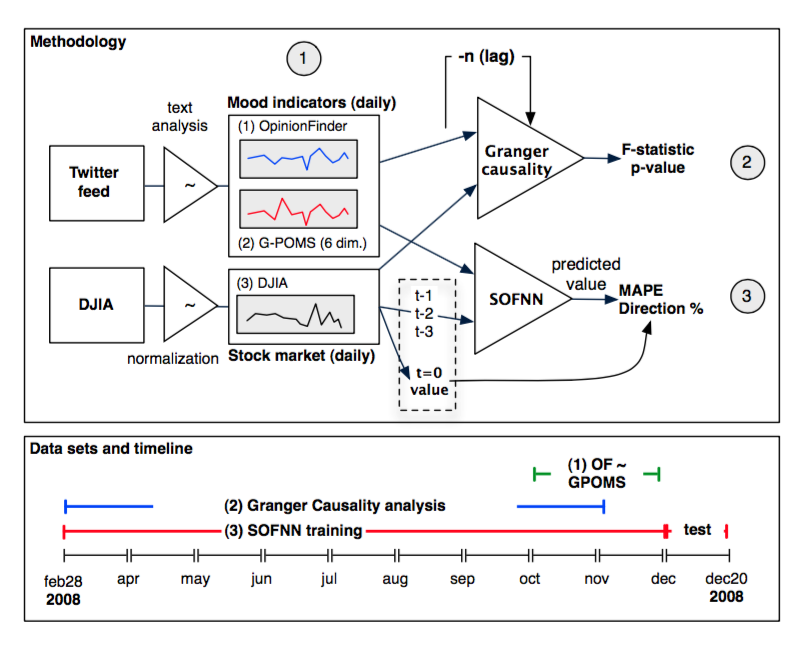
\includegraphics[width=0.5\textwidth]{TwitterPredictionPulibcation.png}
%\end{figure}

\begin{minipage}[b]{0.14\linewidth}
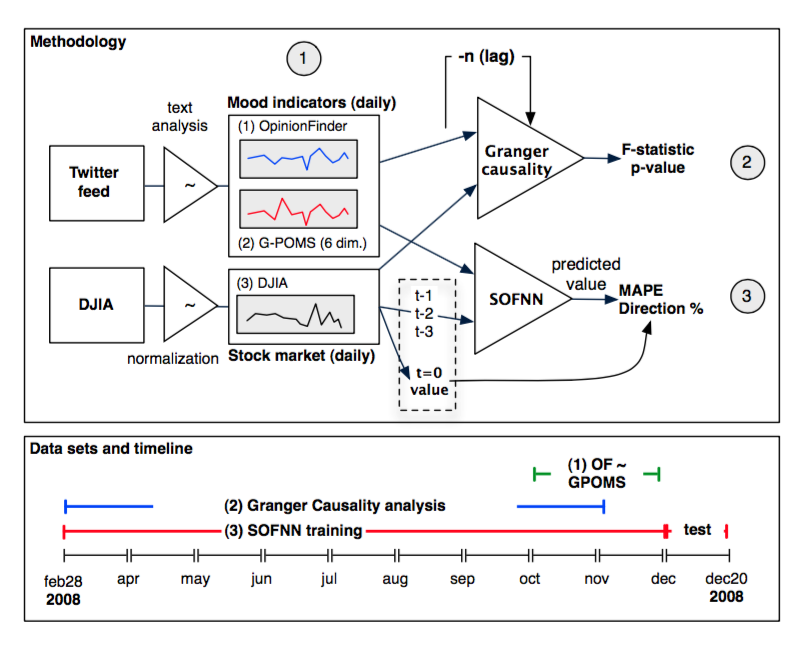
\includegraphics[width=24cm]{TwitterPredictionPulibcation.png} % Logo or a photo of you, adjust its dimensions here
\end{minipage}

%----------------------------------------------------------------------------------------
%	OBJECTIVES
%----------------------------------------------------------------------------------------

\color{DarkSlateGray} % DarkSlateGray color for the rest of the content

\section*{Main Objectives of this project}


\begin{enumerate}
\item Capture and Clean Tweets
\item Capture Stock Price Data
\item Score Tweets and Merge by Time
\item Granger-Causality Test and Analysis
\end{enumerate}

%----------------------------------------------------------------------------------------
%	MATERIALS AND METHODS
%----------------------------------------------------------------------------------------

\section*{Implementation}

Chosen Social Media: Twitter
 The Twitter API allows user to collect tweets based on different types of filters. I choose to search for tweets that contain keyword, \"stock market\", which is the independent variable in this research. After collecting tweets from API, I proceed data cleaning by converting all files into txt form in order to be scored according to the sentiment analysis wordlist. Then, the stock price in the interval of 1 minutes. The last section is the Granger-causality test and running cross validation to verify the relationship between emotions and stock price.

%------------------------------------------------

\subsection*{Capture and Clean Tweets}




\begin{itemize}
\item The first step in capturing tweets or collecting data is connecting the local user with the Twitter API in order to use the searching function online to capture tweets. Twitter API provides certain functions for public study. After registering an Twitter App online, authorization (handshakes) will request user to allow the access, and then the OAuthFactory function connects the API and store the authorization information to the local file my\_oauth.Rdata.
\\


\begin{knitrout}
\definecolor{shadecolor}{rgb}{0.969, 0.969, 0.969}\color{fgcolor}RT @philstockworld: Monday’s Oil Mess: Rent-A-Rebel Jacks up Prices into the Holiday $USO $AAPL 
#Earnings -- https://t.co/cGHB3WDKA8 https…
\end{knitrout}

\bigskip

\item Then the data capturing process first read the authorization information and stream tweets that contain keywords entered by user in the function filterStream. It stores the data in a local variable called "tweets.json" as the format of streaming is json. Name can be changed while data will be stored additionally with the same name. ParseTweets function convert all tweets collect into a data frame with time, content, user, location etc. 


\item In order to process the tweets we collect, mainly scoring the emotion of each tweet. In the scoring function, we get rid of all special symbols, starting users name,  punctuation, digit, link, capital letter. It will be easier for judging whether one string contains on string. 

\end{itemize}

\subsection*{Capture Stock Price Data}

\begin{itemize}

\item Google provides last 15 days of data with one minutes interval. We only have to construct the url string to access the txt format of table and then format them together. We first go to the url, get organize the data into columns. We then search for the time stamp, which is in POSCIX format. Then we convert it to EST and get two columns from this data frame: price closed and time for the future analysis 
\\

\begin{center}

\begin{knitrout}
\definecolor{shadecolor}{rgb}{0.969, 0.969, 0.969}\color{fgcolor}
\begin{tabular}{l|r|l|r}
\hline
Time2 & summary.score & CLOSE & close\_num\\
\hline
2016-05-17 09:15:00 & -14 & 7896.85 & 7896.85\\
\hline
2016-05-17 09:16:00 & -19 & 7905.8 & 7905.80\\
\hline
2016-05-17 09:17:00 & -20 & 7901.6 & 7901.60\\
\hline
2016-05-17 09:18:00 & -29 & 7902.75 & 7902.75\\
\hline
2016-05-17 09:19:00 & -7 & 7909.1 & 7909.10\\
\hline
2016-05-17 09:20:00 & -27 & 7908.25 & 7908.25\\
\hline
\end{tabular}


\end{knitrout}

\end{center}

\end{itemize}


\subsection*{ Score Tweets and Merge by Time}

\begin{itemize}

\item In the scoring function, we use a for loop to search for the positive or negative word in one specific string. It is fairly easy to achieve by lookup each word in the word list and record number of positive words and negative words and calculate the difference between them. However, we also have to get rid of the repetitive count when two positive words or two negative words contain one of the other. The for loop firstly run through negative words and delete repetitive terms and executes in the same way for positive words. 

\begin{center}

\begin{knitrout}
\definecolor{shadecolor}{rgb}{0.969, 0.969, 0.969}\color{fgcolor}
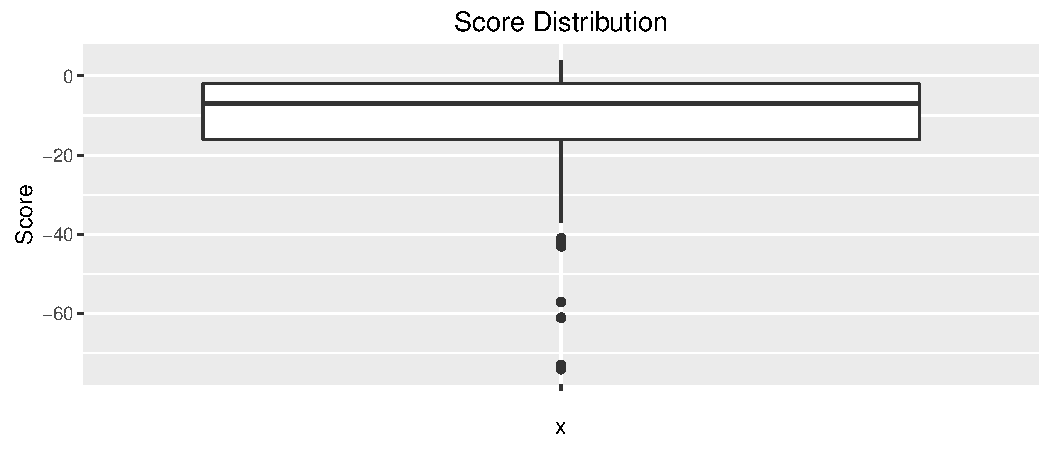
\includegraphics[width=\maxwidth]{figure/myplot-1} 

\end{knitrout}

\end{center}


\item After we put the tweets into a data frame, we then run the clean and score functions to process the information we have. Then merge the score and the price tables by time. Meanwhile, we also make the smallest units to be 1 minutes instead of 1 second because Google data does not provide the instantaneous price. 

\end{itemize}

\subsection*{ Granger-Causality Test and Analysis}

\begin{itemize}

\item Granger Causality Test shows that whether one factor is the predictive factors of another. It uses one factor at first then use two factors to see the correlation between two polynomials by F test. The result will show R square, the percentage of data or correlation that can be explained. It will tell whether a factor is significant predictive factor of the other. In this test, we want to see whether emotion is the deterministic factor of the stock price. We only have to assign our previous two columns to be time series data and run the Granger-causality test code. 
\\

\begin{center}

\begin{knitrout}
\definecolor{shadecolor}{rgb}{0.969, 0.969, 0.969}\color{fgcolor}
\begin{tabular}{l|l|l}
\hline
ftest & p.value & R.squared\\
\hline
40.351 & 6.56e-10 & 0.261\\
\hline
\end{tabular}


\end{knitrout}

\end{center}

\end{itemize}




%----------------------------------------------------------------------------------------
%	RESULTS 
%----------------------------------------------------------------------------------------


%----------------------------------------------------------------------------------------
%	CONCLUSIONS
%----------------------------------------------------------------------------------------

\color{SaddleBrown} % SaddleBrown color for the conclusions to make them stand out

\section*{Results and Conclusions}

\item After running Granger causality test the 10 days interval data, the p-value is $9.03*10^{-11}$ and the $R^2$ is around 0.26. It indicates that there is an moderate correlation between emotional factors and stock market price from the perspective of this research. There is still room for many improvements. 

\color{DarkSlateGray} % Set the color back to DarkSlateGray for the rest of the content

%----------------------------------------------------------------------------------------
%	FORTHCOMING RESEARCH
%----------------------------------------------------------------------------------------

\section*{Forthcoming Research}

The next stage of the research will be improving dictionary by adapting a wordlist that differentiates the emotional level of the words. Or using machine learning to analyze the emotion by Google Opinion Finder. The keywords search also needs improvement as "stock market" is not the only thing that is related to the stock market. A specific company analysis may also be run considering the public exposure of each company is different. 
The program is also expected to run the analysis test and prediction at the same time for potential contribution to the trading strategy


 %----------------------------------------------------------------------------------------
%	REFERENCES
%----------------------------------------------------------------------------------------

\nocite{*} % Print all references regardless of whether they were cited in the poster or not
\bibliographystyle{plain} % Plain referencing style
\bibliography{sample} % Use the example bibliography file sample.bib

%----------------------------------------------------------------------------------------
%	ACKNOWLEDGEMENTS
%----------------------------------------------------------------------------------------

\section*{Acknowledgements}

I am thankful to PRISMS for providing time and support for my endeavors. The algorithm was implemented in R language \cite{Rlang}.
%----------------------------------------------------------------------------------------

\end{multicols}
\end{document}
